\chapter{Primal-Dual algorithm}
\label{cha:pdalgo}


In this chapter we talk about matching problems, a very
important topic in combinatorial optimization.

\section{Graphs and Matchings}
\label{sec:gandm}

%Recall the following definitions, which will be very useful in this 
%chapter.

%\begin{definition}[Undirected Graph]
%   An \emph{undirected graph} $G=(V,E)$ consists of a set $V$
%   of  \emph{vertices} (also called \emph{nodes}) and a set 
%   $E$ of \emph{edges}. An edge $e=\{u,v\}$ is a 
%   2-elements subset of $V$, where $u$ and $v$ are called the 
%   \emph{endpoints} of $e$. 
%\end{definition} 

%\begin{definition}[Directed Graph]
%   A \emph{directed graph} (also called \emph{digraph)} $G=(V,A)$ 
%   consists of a set $V$ of  \emph{vertices} (also called 
%   \emph{nodes}) and a set $A$ of \emph{arcs}. An arc $a$ is an 
%   ordered pair $(u,v) \in V\times V$, where $u$ and $v$ are called 
%   the \emph{tail} and the \emph{head} of $a$ respectively. 
%   Moreover $u$ and $v$ are also called the \emph{endpoints} of $a$.
%\end{definition} 

We begin by giving some useful definitions.

\begin{definition}
   A graph $G=(V,E)$ (or $G=(V,A)$) is called \emph{bipartite} 
   if we can split $V$ into two disjoint subsets $V_1$ and $V_2$,
   such that for every $e \in E$ (or $a \in A$) one endpoint is
   in $V_1$ and the other one is in $V_2$.
\end{definition}


We recall an important result about bipartite graphs.

\begin{lemma}
   A graph is bipartite if and only if it does not contain
   an odd cycle (that is, a cycle of odd length).
\end{lemma}

\begin{definition}[Matching]
   Let $G=(V,E)$, or $G=(V,A)$, be a graph. A \emph{matching} 
   in $G$ is a subset $M \subseteq E$, or $M \subseteq A$, of
   pairwise disjoint edges, or arcs (that is, edges, or arcs,
   which do not share any vertex).
   A vertex $v$ that is an endpoint of an edge (or arc) in 
   $M$ is called a \emph{matched node}, otherwise it is 
   called an \emph{exposed node}.
   A matching is called \emph{perfect} if there are no
   exposed nodes.
\end{definition}

\begin{definition}
   Let $G=(V,E)$ be a graph and $M \in E$ be a matching in $G$.
   An \emph{alternating path} is a path that alternates between
   edges in $M$ and edges in $E \backslash M$. An alternating
   path that starts and ends at an exposed node is called an
   \emph{augmenting path}.
\end{definition}

\begin{definition}[Vertex cover]
   Let $G=(V,E)$ be a graph. A \emph{vertex cover} is a
   set $C \subseteq V$ such that every $e \in E$ has at least
   one endpoint in $C$.
\end{definition}

\begin{figure}[htbp]
  \begin{center}
   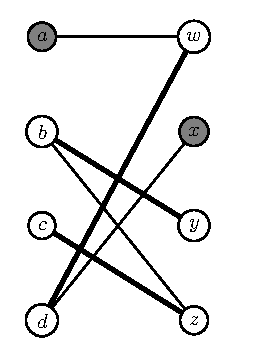
\includegraphics{figures/bipartite-graph.pdf}
  \end{center}
    \caption{This picture shows an example of an undirected
    bipartite graph $G=(V,E)$, where $V = \{a,b,c,d,w,x,y,z\}$,
    $E=\{\{a,w\},\{b,y\},\{b,z\},\{c,z\},\{d,w\},\{d,x\}\}$,
    $V_1=\{a,b,c,d\}$ and $V_2=\{w,x,y,z\}$. 
    The thicker edges form a matching, vertices $a$ and $x$ 
    (marked in grey) are exposed nodes and $a,w,d,x$ is an 
    alternating and augmenting path. $C=\{b,w,x,z\}$ is a vertex 
    cover.}
    \label{fig:bipgraph}
\end{figure}

\section{Matching problems}
\label{sec:matprob}

Now that we know some basic definitions, we can
concentrate on two of the most important problems about
matchings:
\begin{enumerate}
   \item \textbf{Maximum cardinality matching problem}:
    Find a matching $M$ of maximum size.
   \item \textbf{Maximum (or minimum) weight matching problem}:
   Given a graph $G=(V,E)$ and a weight function 
   $w:~E\longrightarrow\setR$, find a matching $M$ of maximum
   (or minimum) weight, where the weight of a matching is
   \begin{displaymath}
        w(M) = \sum_{\substack{e \in M}}  w(e). 
   \end{displaymath}
\end{enumerate}

From now we will focus on the case of an undirected bipartite 
graph $G=(V,E)$.

\subsection{The maximum cardinality matching problem}
\label{subsec:maxcarmat}

Before giving a method to find a maximum cardinality matching
in a graph, we want to show how we can prove its optimality. 
For this purpose we recall theorem~\ref{thr:16}, that gives
an upper bound on the size of any matching in a given bipartite
graph, and we prove another theoreme, which gives us a method
to see if a matching is of maximum size or not.

\begin{theorem}[K\"onig's theorem]
   In any bipartite graph, the number of edges in a 
   maximum cardinality matching equals the number of vertices in 
   a minimum vertex cover. 
\end{theorem}

\begin{theorem}
   A matching $M$ of a graph $G=(V,E)$ is of maximum 
   cardinality if and only if there are no augmenting paths
   with respect to $M$.
\end{theorem}

\begin{proof}
   $(\Rightarrow)$ Suppose there exists an augmenting path in
   $G$, call it $P$. Consider the set $M' = M \triangle P$.
   By definition of augmenting path, we have that $M'$ has
   exactly one edge more than $M$. Since $M$ is a matching
   and $P$ starts and ends in an exposed node, the only edges
   of $M$ with an endpoint in $P$ are the edges of $P$. This implies
   that $M'$ is a matching.
   
   $(\Leftarrow)$ Let $M$ be a maximum cardinality matching
   and let $\tilde{M}$ be a strictly smaller matching.
   Consider $X=M \triangle \tilde{M}$. $X$ is formed by
   cycles and alternating paths (with respect to $M$ and
   $\tilde{M}$). Since $ |M| \textgreater
   |\tilde{M}|$, $X$ contains at least one alternating 
   path $P$ with more edges from $M$ than from $\tilde{M}$.
   By definition of $X$, we see that $P$ is an 
   augmenting path. \qed
\end{proof}

We are now ready to show an algorithm that allows us to
find a maximum cardinality matching in any bipartite graph.

Let $G=(V,E)$ be a bipartite graph with bipartition 
$V = A \sqcup B$ and $M$ a matching.
Now turn $G$ into a directed graph $D=(V,A)$ by directing 
matching edges from $A$ to $B$ and non-matching edges from $B$ to $A$.
We are interested in a method to find augmenting paths or to
assert that there aren't any (and thus, that $M$ is of 
maximum size). For this purpose we illustrate the following
claim and theorem.

\begin{claim}
   Let $G$ and $D$ be as above.
   A path in $D$ between two exposed nodes that starts in
   an exposed node in $B$ (resp. in $A$), ends in an exposed 
   node in $A$ (resp. in $B$).   
\end{claim}

\begin{theorem}
   Let $G$ and $D$ be as above and $M$ be a matching.
   There exists an augmenting path in $G$ if and only if 
   there exists a path from an exposed node in $B$ to an
   exposed node in $A$ in the directed graph $D$.
\end{theorem}

\begin{proof}
   $(\Rightarrow)$ This is a direct consequence of the choice
   of the direction of the arcs in $D$ and of the previous 
   claim.
   
   $(\Leftarrow)$ Trivial.
\end{proof}

Let $G$ and $D$ be as illustrated before.
How can we use the previous theorem for our purpose?  
Add a vertex $s$ to our directed graph $D$ and connect it to all 
exposed nodes in $B$ by an arc whose tail is $s$. 
Now we have that finding a directed path, in $D$, from an exposed 
node $u$ in $B$ to an exposed node $v$ in $A$ is equivalent 
to finding a directed path from $s$ to $v$ passing by $u$. 
Thus, we deduce that there is an augmenting path in $G$ if and 
only if there is at least one exposed node in $A$ reachable from $s$. 
To find if there are such nodes reachable from $s$ and the 
corresponding augmenting paths, we can use the 
\emph{Breadth-First search} algorithm (see chapter~\ref{subsec:BFs}) 
applied to vertex $s$ in $D$.
If there is any exposed node $u$ in $A$ with finite distance 
from $s$, then we can obtain an augmenting path by taking
the shortest path $s,a_1,a_2,\cdots,u$ from $s$ to $u$
(which is given by Bread-First search) without $s$ (i.e., the augmenting path would be $a_1,a_2,\cdots,u$).

To resume, we obtain the following algorithm.

\begin{algorithm}
  \begin{tabbing}
     \\
     {\bf Initialise} \= $M = \emptyset$  \\
     {\bf while}      \=  $There$ $exists$ $M$-$augmenting$
                          $path$        \\  
                      \>  $Update$ $M$  \\
     {\bf return}     \= $M$ 
  \end{tabbing}
\end{algorithm}

Finally, we are interested in the running time of our algorithm.

\begin{theorem}
   A maximum cardinality matching in a bipartite graph 
   $G=(V,E)$ can be computed in time $O(|V| \cdot (|V|+|E|))$.
   If we assume that $G$ does not have any isolated vertex,
   then we can consider the running time to be 
   $O(|V| \cdot |E|)$.
\end{theorem}

\begin{proof}
   The \emph{while loop} runs at most $|V|/2$ times and its
   execution requires $O(|V|+|E|)$ 
   ($=O(|E|)$ if we have the assumption) operations.
\end{proof}

\begin{figure}[htbp]
  \begin{center}
   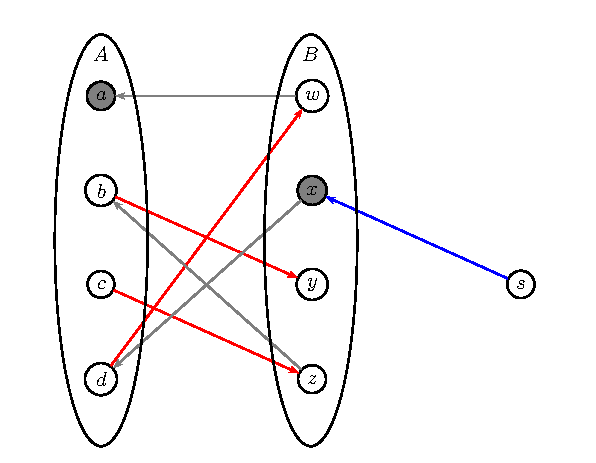
\includegraphics{figures/augpath.pdf}
  \end{center}
    \caption{This picture illustrate how transform a bipartite
    graph to apply the \emph{maximum cardinality matching 
    algorithm}, using the graph of figure~\ref{fig:bipgraph} as
    an example.}
    \label{fig:augpath}
\end{figure}

\subsection{The maximum weight matching problem}
\label{subsec:maxwmat}

In this section we consider a graph $G=(V,E)$ and a weight 
function $w:~E\longrightarrow\setR$. First of all, notice that,
by changing the sign of the weights of all edges, we have that 
finding a maximum weight matching or a minimum weight matching
are equivalent problems.
 
We can also prove 
that the problem of finding a minimum weight matching
can always be replaced by the problem of finding a minimum 
weight \emph{perfect} matching. To see that, it is 
sufficient to create a copy $G'$ of our graph $G$ and add
edges of weight $0$ connecting all vertices $v$ in $G$
to their copy $v'$ in $G'$. This will give us a new graph
$\tilde{G}$. Notice that $\tilde{G}$ has at least a perfect
matching, thus there is one, call it $\tilde{M}$, of minimum 
weight.
If we consider only the edges of $\tilde{M}$ in $G$, we obtain
a minimum weight matching in $G$.

Moreover, we have an important relation between the difficulty
of this two problems, given by the following theorem.

\begin{theorem}
   If there exists a polynomial time algorithm for the minimum
   weight perfect matching problem, then there exists a polynomial 
   time algorithm for the minimum weight matching problem.
\end{theorem}

\begin{proof}
   Let $G=(V,E)$ be a graph. Using the process described above,
   we create the graph $\tilde{G} = (\tilde{V}, \tilde{E})$.
   Notice that $|\tilde{V}| = 2|V|$ and 
   $|\tilde{E}| = 2|E|+|V|$.
   By hypothesis, we can find a minimum weight perfect 
   matching in $\tilde{G}$ (and thus a minimum weight matching
   in $G$) in time $O((\tilde{V} + \tilde{E})^k) =
                    O((2|V|+2|E|+|V|)^k) = O((|V|+|E|)^{k'})$,
   for some $k,k' \in \setN$ (that is, a polynomial time with 
   respect to the size of $G$).
\end{proof}

Since we concentrate on bipartite graphs, we show
how to reduce the problem of finding a minimum weight 
\emph{bipartite} matching to the problem of finding a minimum
weight \emph{bipartite} perfect matching. Let $G=(V,E)$ be a 
bipartite graph with bipartition $V = A \sqcup B$. We can
suppose w.l.o.g. that $|A| \geq |B|$. If $|A|>|B|$, add a
set $C$ of cardinality $|A|-|B|$ and add edges of weight 
zero connecting all nodes of $A$ to all nodes of $B \cup C$.
Call $G'$ the bipartite graph obtained by this process. Obviously,
$G'$ admits at least one bipartite perfect matching, and thus 
also one of minimum weight, call it $M'$. 
By taking out all edges of weight zero from $M'$, we obtain a
minimum weight bipartite matching in $G$.

Also in this case, we have an important relation between
the difficulty of these two matching problems.

\begin{theorem}
   If there exists a polynomial time algorithm for the minimum
   weight bipartite perfect matching problem, then there exists a 
   polynomial time algorithm for the minimum weight bipartite 
   matching problem.
\end{theorem}

\begin{proof}
   Let $G=(V,E)$ be a bipartite graph with bipartition 
   $V = A \sqcup B$. Construct $G'=(V',E')$ as shown above.
   Notice that $|V'| = 2|A| \leq 2|V|$ and 
   $|E'| = |E| + |A| \cdot (|A|-1) \leq |E| + |V|^2$.
   Hence, by hypothesis, finding a minimum weight bipartite 
   matching in $G$ (by finding a minimum weight bipartite perfect 
   matching in $G'$) can be done in time $O((2|V| + |E| + |V|^2)^k)
   = O((|V|+|E|)^{k'})$, for some $k,k' \in \setN$ (that is, a 
   polynomial time with respect to the size of $G$).
\end{proof}

Let $G=(V,E)$ be a bipartite graph. We have showed that the
problem of finding a maximum weight (bipartite) matching can
be reduced to the problem of finding a minimum weight 
(bipartite) perfect matching. Moreover, if there exists a
polynomial time algorithm to solve the first problem, then 
there exists a polynomial time algorithm to solve the second one.

The following theorem is crucial for the introduction of the
\emph{Primal-Dual algorithm}.

\begin{theorem}[Complementary Slackness]
\label{thr:compslack}
   Let 
   \begin{displaymath}
      \begin{array}{c}
         max \ c^T x \\
         Ax \leq b
      \end{array}
   \end{displaymath}
   be a primal LP and let 
   \begin{displaymath}
      \begin{array}{c}
         min \ b^T y \\
         A^T y = c \\
         y \geq 0
      \end{array}
   \end{displaymath}
   be his dual. Let $x^*$ and $y^*$ be primal and dual feasible
   solutions respectively. Then they are both optimal if and
   only if 
   \begin{displaymath}
      (b - A x^*)^T y^* = 0.
   \end{displaymath}
\end{theorem}

\begin{proof}
   \begin{displaymath}
      \begin{array}{c}
         (b - A x^*)^T y^* = 0 \\
         \Leftrightarrow \\
         y^*_i > 0 \Rightarrow a^T_i x^* = b_i \\
         \Leftrightarrow \\
         b^T y^* = (A x^*)^T y^* = (x^*)^T A^T y^* = c^T x
      \end{array}
   \end{displaymath}
   The result follows from strong duality theorem 
   (theorem \ref{thr:4})
\end{proof}

Let $G=(V,E)$ be a bipartite graph.
In order to prove the next theorem, we need to recall the 
\emph{LP-relaxation} of the minimum weight perfect matching 
problem (we will call it the \emph{dual LP}) and his dual (which 
we will call the \emph{primal LP}).

\begin{displaymath}
   \begin{array}{c c}
   PRIMAL                & DUAL \\
   max \sum_{v \in V} y_v & min \sum_{e \in E} w_e \cdot x_e \\
   \ uv \in E: y_u+y_v \leq w_{uv}  \ &
   \ v \in V: \sum_{e \in \delta(v)} x_e = 1 \ \\
   y \in \setR^{|V|}     & x \geq 0
   \end{array}
\end{displaymath}

\begin{theorem}
\label{thr:optmat}
   Suppose $x^*$ and $y^*$ are feasible solutions of the recalled 
   primal and dual linear programs respectively. 
   Then, they are optimal solutions if and only if
   \begin{displaymath}
      \forall uv \in E: 
      x^*_{uv} > 0 \Rightarrow y^*_u + y^*_v = w_{uv}
   \end{displaymath}
\end{theorem}

\begin{proof}
   The proof follows immediately from theorem~\ref{thr:compslack}.
\end{proof}

Another direct consequence of theorem~\ref{thr:compslack} is 
the following criterion for the optimality of a minimum
weight perfect matching.

Let $y^* \in \setR^{|V|}$ be feasible in the primal LP and 
let $G_{y^*}=(V,E_{y^*})$ be the graph with edge set
\begin{displaymath}
   E_{y^*} = {uv \in E: y^*_u + y^*_v = w_{uv}}
\end{displaymath}
If $G_{y^*}$ has a perfect matching $M$, then $y^*$ and $\chi^M$ 
are optimal solutions of the corresponding linear programs,
In particular, since, by definition of $\chi^M$,
\begin{displaymath}
   \chi^M_{uv} > 0 \Rightarrow y^*_u + y^*_v = w_{uv},
\end{displaymath} 
$M$ is a \emph{minimum weight perfect matching}.

\subsection*{The Primal-Dual Algorithm}
Let $G=(V,E)$ be a complete bipartite graph with bipartition 
$V=A \sqcup B$ and edge weights $w: E \rightarrow \setR$. 
The primal-dual algorithm is a method to find a minimum weight 
matching in $G$.
It starts from a feasible solution $y^*$ of the dual LP recalled 
before theorem~\ref{thr:optmat} (notice that a possible 
choice for an initial feasible solution can always be $y^*$ such 
that $y^*_v$ is equal to $0$ or to the smallest edge-weight in 
the graph in the case it is smaller than $0$) 
and it updates this solution until it is optimal. 
The last question we have to answer is: how do we update $y^*$
in such a way that our algorithm terminates correctly?

Let $G_{y^*}$ be as previously defined and let $M$ be a maximum 
cardinality matching in $G_{y^*}$. Turn $G_{y^*}$ into a directed
graph by orientating the matching edges from $A$ to $B$ and the
non-matching edges from $B$ to $A$ (call this new graph 
$\tilde{G}_{y^*}$). 
Let $M$ be a maximum cardinality matching in $G_{y^*}$.
Let $L \subseteq A \sqcup B$ be the set of vertices reachable 
from the set of exposed nodes of $B$ in the directed graph 
$\tilde{G}_{y^*}$.

\begin{claim}
   $G_{y^*}$ does not contain an edge $uv$ with 
   $u \in A \textbackslash L$ and $v \in B \cap L$.
\end{claim}

\begin{proof}
   Let $uv$ be such an edge. If $uv$ is a non-matching edge, then, 
   since $v \in L$, also $u$ has to be in $L$. Suppose now that 
   $uv$ is a matching edge. Since $v \in L$, there must be a 
   matching edge $\tilde{u}v$ with $\tilde{u} \in L$. This implies 
   that $u = \tilde{u}$ and this leads to a contradiction since 
   $u \not\in L$.
\end{proof}

We want to update our solution $y^*$ in such a way to obtain 
an optimal solution. Let 
$\delta = min\{w_{uv}-y^*_u-y^*_v$ $|$
$uv \in E, u \in A \textbackslash L, v \in B \cap L\}$.
If $y^*$ is not already optimal, then $\delta$ is strictly positive.
This allows us to construct a feasible solution $\tilde{y}$ 
in this way:
\begin{enumerate}[i)]
   \item $\tilde{y}_v = y^*_v + \delta$ if 
         $v \in A \textbackslash L$
   \item $\tilde{y}_v = y^*_v - \delta$ if 
         $v \in B \textbackslash L$
   \item $\tilde{y}_v = y^*_v$ otherwise
\end{enumerate}

This gives us a new graph $G_{\tilde{y}}$. 
Notice that the previous claim shows that all the edges of $M$ 
are in $G_{\tilde{y}}$. 
Furthermore, by the definition of $\delta$, at least one edge 
connecting a node in $A \textbackslash L$ to a vertex in 
$B \cap L$ becomes tight. Thus, $L$ is augmented.
This implies that every time we update our solution there 
are two things that can happen:
\begin{enumerate}[i)]
   \item $G_{\tilde{y}}$ contains an augmenting path with respect 
         to $M$. This allows us to increase our matching.
   \item The set $L$ increases.
\end{enumerate}
Since $V$ is a finite set and by the criterion of optimality 
showed before, we can assert that the Primal-Dual algorithm 
terminates correctly.

We conclude by resuming the algorithm, giving his running time 
and an example, which can be useful to understand better how 
the Primal-Dual algorithm works.

\begin{algorithm}
  \begin{tabbing}
     \\
     {\bf Input:}           \= $A$ $feasible$ $solution$ $y^*$   \\
     {\bf Initialisation:}  \= $Turn$ $G$ $into$ $a$ $directed$ 
                               $graph$                           \\  
     {\bf while}            \= $M$ $is$ $not$ $optimal$          \\                               
                            \> $Compute$ $L$                     \\
                            \> $Let$ $\delta = min\{w_{uv}
                                - y^*_u - y^*_v\}$               \\
                            \>$Update$ $y^*$                     \\
     {\bf return}           \= $M$  
  \end{tabbing}
\end{algorithm}

\begin{theorem}
   The Primal-Dual algorithm runs in $O(|V^2|)$ time.
\end{theorem}

\begin{proof}
   We can have at most $|V|$ many augmentation of $L$ 
   without augmenting $M$ and $M$ can be augmented at most $|V| / 2$ 
   times. 
\end{proof}

Figure~\ref{fig:egprimaldual} shows how to apply Primal-Dual 
algorithm on a complete bipartite graph. 

\begin{figure}[htbp]
   \begin{center}
      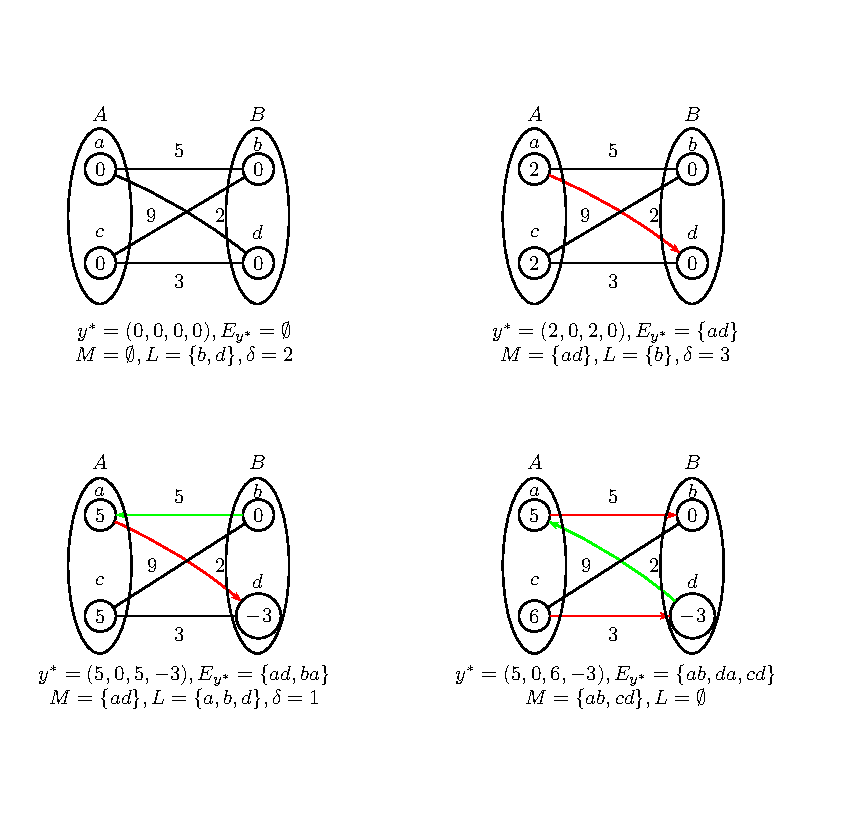
\includegraphics{figures/egprimaldual.pdf}
   \end{center}
 \caption{The edges of $G_{y^*}$ are coloured, red for 
 the matching edges, and green for the non-matching edges.}
 \label{fig:egprimaldual}
\end{figure}

\section*{Exercises} 
\begin{enumerate}
   \item   Let 
           \begin{displaymath}
              \begin{array}{c}
                 max \ c^T x \\
                 Ax \leq b
              \end{array}
           \end{displaymath}
           be a primal LP and let 
           \begin{displaymath}
              \begin{array}{c}
                 min \ b^T y \\
                 A^T y = c \\
                 y \geq 0
              \end{array}
           \end{displaymath}
           be his dual. Let $x^*$ and $y^*$ be primal and dual    
           feasible solutions respectively. Suppose they are
           both optimal. Is the following true: 
           if $a^T_i x^* = b_i$, then $y^*_i > 0$?
           
   \item   Find $G_{y^*}$ from the graph $G=(V,E)$ shown in
           figure~\ref{fig:exgraph} as described in the 
           criterion for the optimality of a minimum
           weight perfect graph.
          
           \begin{figure}[htbp]
             \begin{center}
               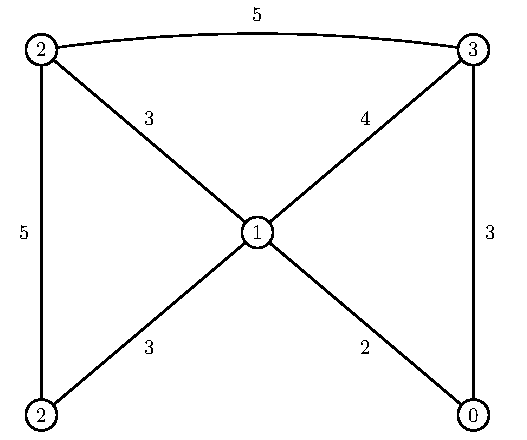
\includegraphics{figures/exgraph.pdf}
             \end{center}
               \caption{$G=(V,E)$}
               \label{fig:exgraph} 
           \end{figure} 
           
   \item   Are there rational numbers $y_1, y_2, y_3, y_4$ such 
           that 
           \begin{displaymath}
              \begin{array}{c}
                 y_1 + y_3 \leq 5 \\
                 y_1 + y_4 = 2 \\
                 y_2 + y_3 = 9 \\
                 y_2 + y_4 \leq 3
              \end{array}
           \end{displaymath}
           
   \item   Apply Primal-Dual Algorithm to the complete bipartite 
           graph of figure~\ref{fig:exprimaldualalgo} (we give 
           an initial feasible solution $y^*=(0,0,0,0)$).
           \begin{figure}[htbp]
             \begin{center}
               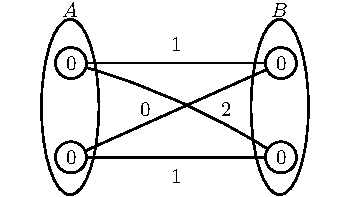
\includegraphics{figures/exprimaldualalgo.pdf}
             \end{center}
             \caption{}
               \label{fig:exprimaldualalgo}
           \end{figure}
           
\end{enumerate}


%%% Local Variables: 
%%% mode: latex
%%% TeX-master: "lecture"
%%% End: 
 